\documentclass[11pt]{article}

% Change "review" to "final" to generate the final (sometimes called camera-ready) version.
% Change to "preprint" to generate a non-anonymous version with page numbers.
% "final" is used here so the author names and IDs are shown.
\usepackage[final]{acl}

% Standard package includes
\usepackage{times}
\usepackage{latexsym}

% For proper rendering and hyphenation of words containing Latin characters (including in bib files)
\usepackage[T1]{fontenc}

% This assumes your files are encoded as UTF8
\usepackage[utf8]{inputenc}

% This is not strictly necessary, and may be commented out,
% but it will improve the layout of the manuscript,
% and will typically save some space.
\usepackage{microtype}

% This is also not strictly necessary, and may be commented out.
% However, it will improve the aesthetics of text in
% the typewriter font.
\usepackage{inconsolata}

%Including images in your LaTeX document requires adding
%additional package(s)
\usepackage{graphicx}

% Tables
\usepackage{booktabs}
\usepackage{float}

\title{The Silent Tax: How Typos Reshape Reasoning in Thinking LLMs}

\author{Shiran Hamami \\ 207487026 \\ \texttt{shiranhamami@mail.tau.ac.il} \And
Dolev Abudi \\ 323096099 \\ \texttt{dolevabudi@mail.tau.ac.il} \AND
Ron Shtricker \\ 209524552 \\ \texttt{ronshtricker@mail.tau.ac.il} \And
Ido Azoulay \\ 212710958 \\ \texttt{idoazoulay1@mail.tau.ac.il}}

\begin{document}
\maketitle
\begin{abstract}
Reasoning models perform strongly on clean mathematical and scientific benchmarks, but real users often write with typos. We study how such errors affect not only final-answer accuracy but also the reasoning process itself. We introduce a controlled typo generator that independently varies the number of corrupted words and the share of typos that produce another valid English word (real-word typos). We apply it to 500 questions from each of GSM8K, MATH-500, and ARC-Challenge and evaluate DeepSeek-R1-Distill-Qwen-7B across all corruption settings. Typos consistently reduce accuracy most on GSM8K, from 92.6\% on clean questions to 64.5\% in the most corrupted setting. At a fixed number of typos, real-word typos are more harmful than non-word ones: about 1.7$\times$ per typo on GSM8K and 1.3$\times$ on MATH-500, while on ARC-Challenge only real-word typos have a detectable effect. The reasoning traces show that the model often notices that something is wrong, but it hesitates more without verifying more. Finally, we introduce three mitigation strategies but none of these simple mitigations (a typo warning, rewriting the question, and spell checking) reliably helps. The main challenge is not detecting corrupted input but recovering its intended meaning.
\end{abstract}

\section{Introduction}

Chain-of-thought prompting and reasoning-focused models have substantially improved performance on mathematical and scientific benchmarks \citep{wei2022,guo2025}. However, benchmark questions are carefully written, while real users often make typing mistakes such as swapped letters, missing characters, or nearby-key errors. Strong performance on clean benchmark text may therefore not fully reflect reliability in real-world use. This gap motivates our study.

Prior work shows that typos hurt LLM performance, especially on reasoning tasks \citep{gan2024,zhao2026}, and attributes part of this sensitivity to subword tokenization \citep{chai2024}. These studies, however, score only final answers and do not analyze what happens inside the reasoning process as a result, reasoning models make this question especially interesting. Their long reasoning traces give them many opportunities to notice a corrupted word, infer what was intended, and recover before producing the final answer. In this study, we also evaluate the reasoning trace itself.

To study this, we created typo generator that separates two factors: how many words are corrupted and what kind of corruption they contain. In particular, we vary the share of typos that accidentally produce another valid real-word. This allows us to investigate and evaluate the difference between real-word and non-word typos while the number of typos stays fixed, a comparison that previous work has not made. We evaluate DeepSeek-R1-Distill-Qwen-7B \citep{guo2025} across the full set of conditions on three datasets with different reasoning characteristics. Beyond measuring final-answer accuracy, we also examine the reasoning traces themselves using word-level alignment and an LLM judge.

Our main contributions are: (i) a controlled experimental setup that independently varies typo rate and the proportion of real-word typos across three datasets; (ii) an analysis of how typos affect the reasoning process itself, including changes in model uncertainty, whether the model notices corrupted words, and whether it attempts to repair them, and (iii) an evaluation of three simple mitigation strategies: warning the model that the input may contain typos, asking it to correct possible typos before solving the problem, and applying an external spell checker before the model sees the question.

Our main findings are as follows. Typos cost up to 28.1 percentage points of accuracy on GSM8K, and the loss comes from wrong answers rather than truncated generations (\S5.1). At a fixed number of typos, real-word typos are more harmful than non-word ones, by 1.3--1.7$\times$ per typo on GSM8K and MATH-500 (MATH-500 only borderline), while on ARC only real-word typos have a detectable effect (\S5.2). Contrary to our initial expectation that real-word typos would pass unnoticed, the model flags corrupted words, and hedges, more often as corruption grows, yet it also misreads more words and does not verify more (\S5.3, \S5.4). Finally, none of the three mitigations reliably recovers the loss (\S5.5).

\begin{figure}[t]
\centering
\footnotesize
\setlength{\fboxsep}{4pt}
\fbox{\begin{minipage}{0.94\columnwidth}
\textbf{Clean (model answers 18, correct)}

\smallskip
\noindent Janet's ducks lay 16 eggs per day. She eats three for breakfast every morning and bakes muffins for her friends every day with four. She sells the remainder at the farmers' market daily for \$2 per fresh duck egg. How much in dollars does she make every day at the farmers' market?

\medskip\hrule\medskip

\textbf{r=25\%, $\rho$=40\% (}model answers 24, wrong\textbf{)}

\smallskip
\noindent Janet's \textbf{duck} lay 16 eggs per \textbf{adqy}. \textbf{Sje} \textbf{east} \textbf{rthere} for breakfast every morning and bakes muffins for \textbf{uher} \textbf{friend} every \textbf{azy} with four. She sells the remainder at the farmers' market daily for \$2 per \textbf{resh} duck egg. How much in dollars does she make every day at the \textbf{faremrs'} market?
\end{minipage}}
\caption{A single GSM8K item under our generator. Numbers and LaTeX are protected; only alphabetic words are corrupted. Four of the ten typos are \emph{real words} (\texttt{eats$\rightarrow$east}, \texttt{ducks$\rightarrow$duck}, \texttt{friends$\rightarrow$friend}, fresh$\rightarrow$resh); the spell checker accepts the first three. The model answers 24 instead of 18.}
\label{fig:example}
\end{figure}


\section{Background and Related Work}

\paragraph{Typo robustness of LLMs.} Prior studies measure final-answer accuracy under typos. \citet{gan2024} adversarially search for up to eight character edits that derail instruction-tuned models on reasoning benchmarks, and \citet{zhao2026} apply random keyboard edits across 18 open models and 12 languages, finding reasoning tasks among the most affected. \citet{chai2024} attribute the damage to subword tokenization, and in concurrent work, \citet{hu2026} link it more specifically to how many of the question's tokens a typo breaks. Yet a typo can also form another valid word, which tokenizes normally but changes the meaning. None of these studies compares real-word and non-word typos on the same words, and none looks inside the reasoning trace to see where the model goes wrong.

\paragraph{Reasoning traces and self-correction.} A reasoning model could, in principle, notice and repair a typo while it thinks. Concurrent work supports this: a thinking budget recovers almost all of the accuracy lost to keyboard typos \citep{hu2026}. This evidence comes from final accuracy alone. The traces are not examined, so it remains unknown whether the model actually repairs the typos or reaches the answer despite them. Repair is also not guaranteed. On flawed input, reasoning models write much longer, redundant traces rather than resolving the problem \citep{fan2025}, LLMs struggle to correct themselves without external feedback \citep{huang2024}, and a written trace need not reflect the model's actual reasoning \citep{turpin2023}.

\paragraph{Simple fixes.} Repairing the input before reasoning, with a separate model, with the LLM itself, or with a spell-checker, gives mixed results \citep{pruthi2019,wang2024,mu2026,zhu2026}. Spell-checking in particular can pick fluent but wrong dictionary words \citep{zhu2026}, since a dictionary lookup cannot flag a typo that is itself a valid word \citep{kukich1992}; how these fixes behave as such typos become more common has not been measured.


\section{Method}


\subsection{Controlled typo generation}

We generate corrupted versions of each question by modifying only its natural-language text. Numbers, LaTeX expressions, and LaTeX command names are protected and never modified. Candidate words must consist only of ASCII letters, and we exclude single-character words and a small set of common function words.

The generator varies two factors independently. The typo rate r determines how many eligible words are corrupted, while the real-word ratio $\rho$ determines the target fraction of those corruptions that should result in another valid English word (see Figure 1 for an example).

Each corrupted word receives one of four keyboard edits: adjacent-key substitution (probability 0.40), deletion (0.20), insertion (0.20), or transposition (0.20). With probability 0.10, a second edit is applied to the same word.

For each question, we convert $\rho$ into a target number of real-word typos, using probabilistic rounding when the target is not an integer. We then process the selected words in random order. While the target has not been reached, the generator searches for valid real-word variants using the NLTK English lexicon \citep{bird2009}. If none exists for a selected word, that word receives a non-word typo and the generator continues trying to satisfy the target with the remaining words. Any real word produced accidentally is counted toward the target. Because the selected words are not chosen based on whether a real-word variant exists, the requested ratio cannot always be reached exactly. In these cases, the generator gets as close to the target as the selected words allow. Table 1 reports the achieved ratios.

For each benchmark, we compare the clean setting with nine corrupted conditions, described as follows: each condition combines a typo rate r $\in$ \{25, 50, 75\}\% with a real-word ratio $\rho$ $\in$ \{10, 40, 70\}\%. All conditions use the same questions and the same random seed, which allows paired comparisons. The resulting datasets are available on Hugging Face.


\subsection{Datasets}

We use 500 questions from each of three benchmarks: GSM8K \citep{cobbe2021}, MATH-500 \citep{hendrycks2021,lightman2024}, and ARC-Challenge \citep{clark2018}. GSM8K contains arithmetic word problems written mostly in words, with relatively few numbers, so each question has many words that can be corrupted. MATH-500 contains shorter competition problems with substantial LaTeX content, which our generator protects, so its questions have fewer words that are eligible for typos. ARC-Challenge contains short multiple-choice science questions, whose answer options may help the model interpret a corrupted question.

As a result, the same typo rate does not produce the same absolute number of typos across datasets: GSM8K receives the most corruption per question (Table 1).

\begin{table}[t]
\centering
\small
\resizebox{\columnwidth}{!}{%
\begin{tabular}{lrrr}
\toprule
 & GSM8K & MATH-500 & ARC-C \\
\midrule
questions & 500 & 500 & 500 \\
mean words per question & 45.8 & 31.5 & 23.5 \\
median words per question & 43 & 26 & 20 \\
eligible words per question & 30.6 & 15.7 & 16.6 \\
typos per question, r=25\% & 7.6 & 4.0 & 4.2 \\
typos per question, r=50\% & 15.3 & 7.9 & 8.3 \\
typos per question, r=75\% & 22.9 & 11.8 & 12.4 \\
achieved real-word ratio, $\rho$=10\% & 0.100 & 0.099 & 0.102 \\
achieved real-word ratio, $\rho$=40\% & 0.399 & 0.397 & 0.401 \\
achieved real-word ratio, $\rho$=70\% & 0.698 & 0.681 & 0.682 \\
total corrupted words & 68,739 & 35,685 & 37,248 \\
\bottomrule
\end{tabular}}
\caption{Dataset and corruption statistics over the nine corrupted conditions (r $\in$ \{25, 50, 75\}\%, $\rho$ $\in$ \{10, 40, 70\}\%), first 500 questions of GSM8K and ARC-Challenge and all of MATH-500. \emph{Eligible words} are those the generator may corrupt, after protected spans, single-character words and function words are removed; the typo rate applies to them, and real-word ratios are pooled over all corrupted words.}
\label{tab:1}
\end{table}


\section{Experimental Setup}

\paragraph{Models.} We use DeepSeek-R1-Distill-Qwen-7B \citep{guo2025}, accessed through the Hugging Face API, with temperature 0.6 and top-p 0.95 (the model-card defaults, to reflect how a typical user would run it) and one response per question. For the LLM-based evaluation we use Llama-3.3-70B-Instruct \citep{grattafiori2024}, also through the Hugging Face API, with temperature 0.

\paragraph{Prompts.} For math problems, we provide the question followed by the instruction: ``Please reason step by step, and put your final answer within \texttt{\textbackslash{}boxed\{\}}.'' For multiple-choice questions, we present the four answer options with shuffled labels and ask the model to return the final answer as a boxed letter. Typos are added only to the question itself, while the instruction remains unchanged.

\paragraph{Scoring.} We extract the final answer only from the text produced after the closing \texttt{\textless{}/think\textgreater{}} tag. Responses that reach the token limit\footnote{We cap generation at 20,000 tokens for GSM8K and 17,000 for MATH-500 and ARC-Challenge. We chose these limits mainly to remove outlier questions whose reasoning exceeds that length.} without producing a final answer are marked as unanswered (Appendix F). GSM8K is evaluated using normalized numeric matching, MATH-500 using symbolic equivalence with \texttt{math\_verify}, and ARC using exact answer-letter matching. We report accuracy over answered questions together with the number of answered responses, and check the effect of truncation with strict accuracy, which counts unanswered responses as wrong.

\paragraph{Statistics.} Since each condition contains the same 500 questions, we use paired tests. We count the questions that change from correct to incorrect and from incorrect to correct, and compare these paired outcomes with a continuity-corrected McNemar test, which separates the effect of typos from differences in question difficulty.

\paragraph{Reasoning trace analysis.} We analyze the reasoning traces in three ways. First, word-level alignment tracks how the model handles each corrupted word: whether the trace uses the original word, the corrupted form, or both, classifying each typo as silently fixed, flagged, misread, or not used (\S5.3). Second, we measure self-doubt directly from the reasoning traces. We define sets of words and phrases associated with uncertainty and self-correction, and count how often they appear in each trace. Since traces differ in length, we normalize these counts by trace length. We then compare these measures across typo conditions and between correct and incorrect answers to examine whether higher uncertainty is associated with model failure (\S5.4). Third, an LLM judge \citep{zheng2023} receives the list of corrupted words with their originals, the question as shown to the model, and the reasoning trace (its first and last 2,000 characters). Using a fixed rubric, it assigns a \emph{self-doubt} score from 0 (a clear, straight-line solution) to 10 (pervasive uncertainty, reversals or looping), and a \emph{repair} score from 0 (the intended meaning of the question is fully understood) to 5 (the model reasons from the wrong meaning). Higher is worse on both scales. The judge scores answered traces only.


\section{Results}


\subsection{Effect of typos on accuracy}

\begin{figure*}[t]
\centering
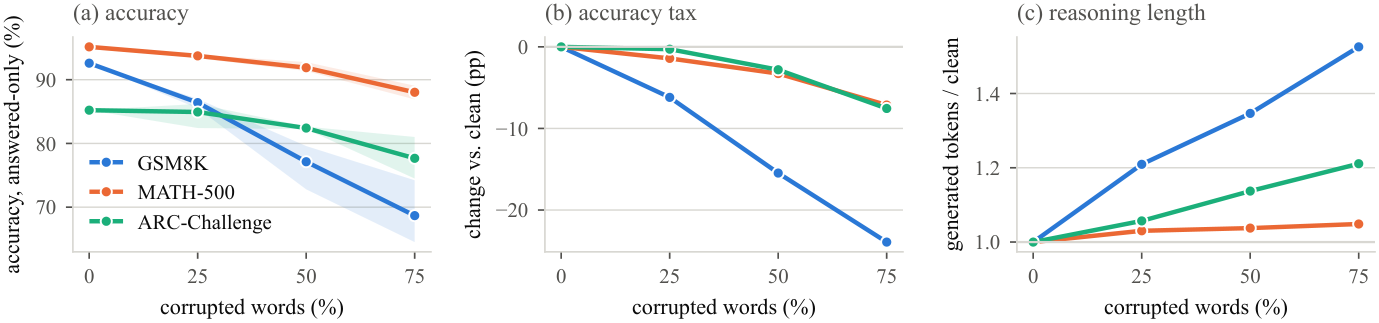
\includegraphics[width=\textwidth]{figures/fig2_accuracy.png}
\caption{\textbf{The accuracy tax.} \emph{(a)} answered-only accuracy against the typo rate; the line is the mean over the three real-word ratios and the band spans them. \emph{(b)} the same as a change from clean, in percentage points. \emph{(c)} mean generated tokens relative to clean. Accuracy falls with the typo rate on all three datasets and falls fastest on GSM8K, where the text carries the whole problem. On average, reasoning gets longer under typos, so the loss is not the model giving up early.}
\label{fig:2}
\end{figure*}

Figure 2 and Table 4 in the appendix show the full results. On GSM8K, answered-only accuracy drops from 92.6\% on clean questions to 64.5\% in the most corrupted condition (r=75, $\rho$=70). ARC drops from 85.2\% to 74.5\%, and MATH-500 from 95.2\% to 86.9\%. On all three datasets accuracy is lowest at the highest typo rate, although on ARC the mildest rate (r=25) is still on par with clean.

The paired analysis shows the same trend. In the most corrupted GSM8K condition, 148 questions change from correct to incorrect, while only 11 change from incorrect to correct, out of 482 questions answered in both conditions (p $<$ 10$^{-6}$). ARC shows 77 correct-to-incorrect versus 25 incorrect-to-correct changes, and MATH-500 shows 46 versus 7, both statistically significant. GSM8K is affected even at the mildest typo condition, while significant effects appear only at higher typo rates for MATH-500 and ARC (Table 4). One possible explanation is how much each task depends on the wording of the question: GSM8K problems rely on the text to describe the quantities and relationships needed for the solution, ARC's answer options may help the model recover some information, and much of the mathematical content of MATH-500 is written in protected LaTeX.

Typos also lead to longer reasoning traces across all three datasets, while the model still produces final answers in most cases. On GSM8K accuracy falls from 92.6\% to 62.2\%; of this strict drop at r=75, $\rho$=70, 92\% comes from answered-but-wrong responses and only 8\% from truncation, and on MATH-500 truncation contributes nothing and on ARC 5\%. Typos also lengthen the reasoning: on GSM8K the mean trace grows from 1,535 tokens on clean questions to 2,330 in the most corrupted condition (and up to 2,593 at r=75, $\rho$=40), with smaller increases on MATH-500 and ARC. This suggests that the drop in accuracy is driven mainly by incorrect answers rather than incomplete generations. In fact, wrong answers tend to have longer reasoning traces than correct ones, indicating that additional reasoning is more closely associated with difficulty than with successful recovery (Figure 2c; Table 7).


\subsection{Real-word typos are more harmful}

\begin{figure}[t]
\centering
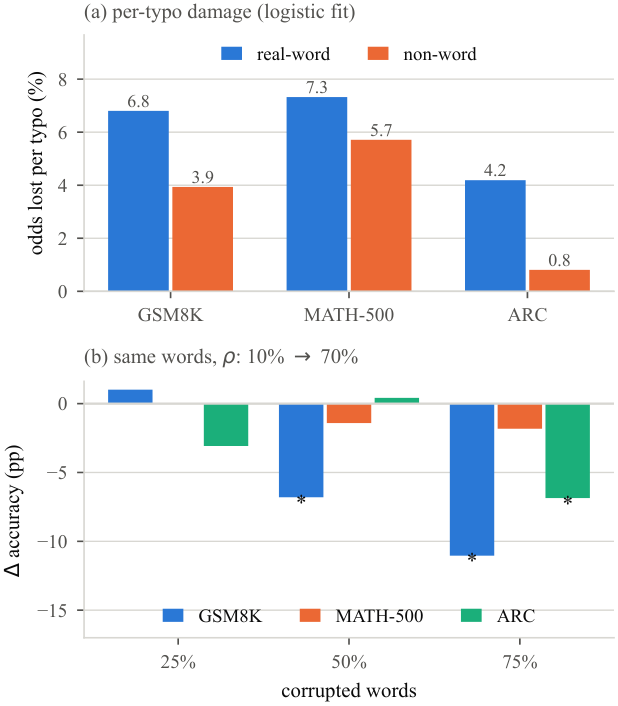
\includegraphics[width=\columnwidth]{figures/fig3_realword.png}
\caption{\textbf{The real-word effect.} \emph{(a)} multiplicative loss in the odds of a correct answer per additional typo, from a logistic regression fitting real-word and non-word counts separately. \emph{(b)} the controlled paired comparison: the same questions with the same number of typos, changing only the real-word share from $\rho$=10 to $\rho$=70. * marks McNemar p$<$0.05.}
\label{fig:3}
\end{figure}

Because typo rate and real-word ratio are varied independently, we can compare real-word and non-word typos while controlling for the total number of typos. For each dataset, we fit a logistic regression using the number of real-word and non-word typos to predict whether the final answer is correct (Figure 3a). The results show that an additional real-word typo has a stronger negative association with correctness than an additional non-word typo: the relative per-typo loss is about 1.7$\times$ larger on GSM8K (95\% CI 1.4--2.3), 1.3$\times$ on MATH-500 (1.0--1.7, only borderline), and 5.2$\times$ on ARC, but ARC's non-word coefficient is not distinguishable from zero, so its ratio is not well defined (Table 5).

The paired comparisons support this pattern, although the effect depends on the overall typo rate. On GSM8K at a 75\% typo rate, increasing the real-word share from 10\% to 70\% lowers accuracy by 11.0 percentage points, even though the same questions contain the same total number of typos. The difference is also significant at a 50\% typo rate, but not at 25\%. When corruption is mild, the model can often handle both kinds of typo, and the difference becomes more pronounced as the overall typo rate increases (Figure 3b; Table 6). ARC shows a significant real-word effect at the highest typo rate, while MATH-500 shows no significant difference at any typo rate, consistent with its smaller number of corrupted words.

Overall, real-word typos can be especially difficult for the model. Unlike non-word typos, which produce visibly unusual word forms, they result in valid words and can change the meaning of the input without creating an obvious tokenization problem.


\subsection{Repair behavior: noticed but not repaired}

\begin{figure*}[t]
\centering
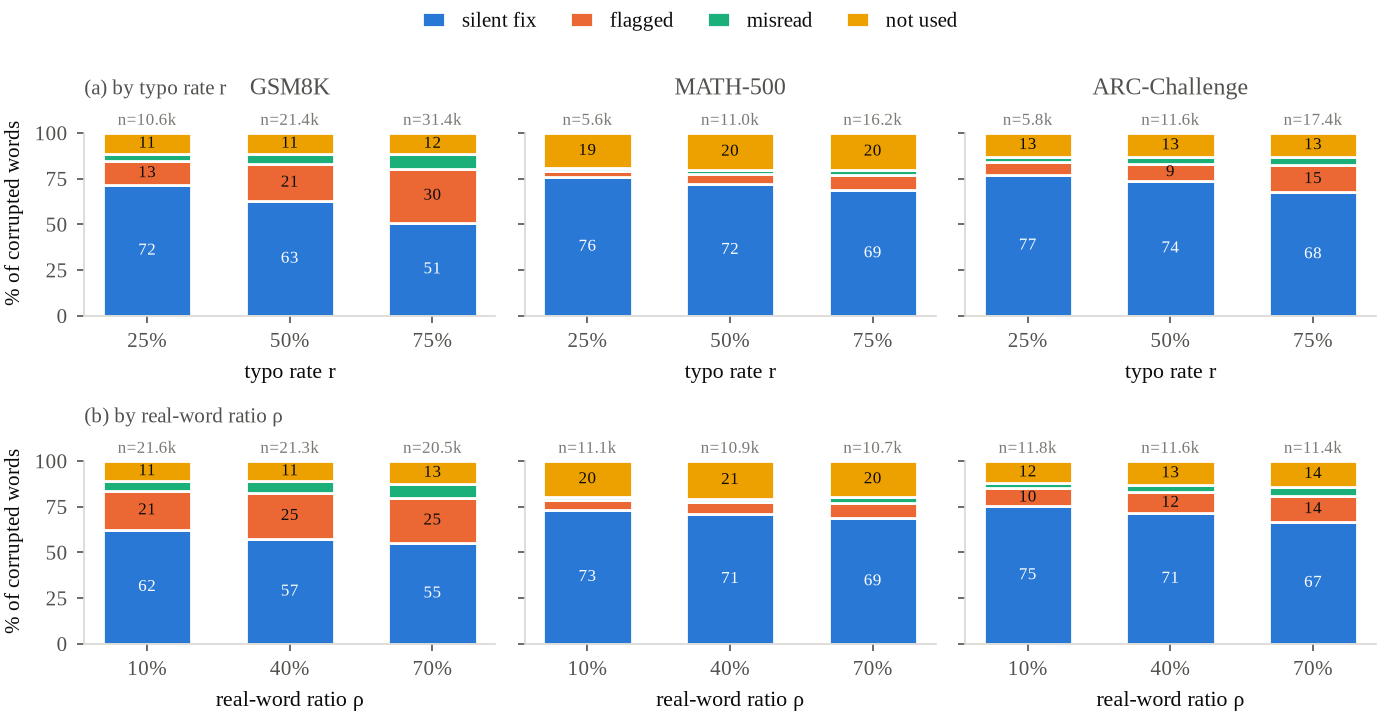
\includegraphics[width=\textwidth]{figures/fig4_repair.png}
\caption{\textbf{Word-level repair behavior.} Each bar is 100\% of the corrupted words in the conditions it pools (n above the bar, in thousands of words). The x-axis sets how many words are corrupted; the segments split those corrupted words by how the reasoning trace handles them. For example, at r=25\% on GSM8K, 25\% of the eligible words in each question are corrupted, and 72\% of those corrupted words are silently fixed. \emph{(a)} by typo rate r, pooled over real-word ratios. \emph{(b)} by real-word ratio $\rho$, pooled over typo rates. Segments below 9\% are not labeled; per-condition values are in Table 8.}
\label{fig:4}
\end{figure*}

We recover each corrupted word by comparing the clean and corrupted versions of the question, and classify how the model handles it in the reasoning trace: \textbf{silent fix}, only the original word appears (the model recovered the intended word without mentioning the typo); \textbf{flagged}, both the original and the corrupted form appear (the model noticed and corrected the typo); \textbf{misread}, only the corrupted form appears (the model took it as the wrong word); and \textbf{not used}, neither form appears.

We originally expected real-word typos to go unnoticed more often, while non-word typos would be easier to detect and correct explicitly. The results only partly support this prediction. As the typo rate increases from 25\% to 75\%, silent fixing decreases on all three datasets; on GSM8K, for example, it falls from 74.0\% to 55.8\% at $\rho$=10. At the same time, flagging and misreading become more common: pooled over real-word ratios, misreading rises from 3.9\% to 7.8\% on GSM8K and from 1.4\% to 2.7\% on MATH-500, and less steeply on ARC, from 2.9\% to 4.6\% (Figure 4; Table 8).

Increasing the real-word ratio has a similar effect. Pooled across typo rates on GSM8K, silent fixing falls from 62.4\% to 55.3\% as $\rho$ increases from 10 to 70, while flagging rises from 21.4\% to 24.5\% (levelling off above $\rho$=40) and misreading from 5.2\% to 7.5\%; the same overall pattern appears on MATH-500 and ARC. Misreading is also related to failure: in every condition it is 1.2 to 2.0 times more frequent in GSM8K traces that end in a wrong answer, and 1.3 to 2.7 times on ARC; on MATH-500, where misreads are rare, the relation is not consistent (Table 8). The share of typos that are not used stays stable within each dataset but differs across tasks, roughly 12\% on GSM8K, 13\% on ARC, and 20\% on MATH-500, possibly because MATH-500 reasoning is more symbolic and refers back to the wording of the question less often.

The judge's repair score (\S4; Table 2) tells the same story. It rises with the typo rate (on MATH-500 only at r=75), and wrong answers score higher than correct ones (over the typo conditions: 2.40 vs. 0.97 on GSM8K), linking misunderstanding of the corrupted question to failure. It also rises with the real-word ratio in every dataset and typo-rate cell, consistent with real-word typos being harder to repair, although we did not test this trend for significance.


\subsection{Self-doubt}

\begin{table}[t]
\centering
\small
\resizebox{\columnwidth}{!}{%
\begin{tabular}{lrrrrrr}
\toprule
 & \multicolumn{2}{c}{\textbf{GSM8K}} & \multicolumn{2}{c}{\textbf{MATH-500}} & \multicolumn{2}{c}{\textbf{ARC-C}} \\
\cmidrule(lr){2-3}\cmidrule(lr){4-5}\cmidrule(lr){6-7}
\textbf{condition} & repair & doubt & repair & doubt & repair & doubt \\
\midrule
\multicolumn{7}{l}{\emph{clean}} \\
--- & 0.12 & 4.46 & 0.03 & 3.66 & 0.03 & 4.70 \\
\multicolumn{7}{l}{\emph{by typo rate} r} \\
25\% & 0.88 & 4.86 & 0.35 & 3.90 & 0.97 & 5.12 \\
50\% & 1.27 & 5.12 & 0.35 & 3.98 & 1.03 & 5.31 \\
75\% & 1.74 & 5.67 & 0.48 & 4.01 & 1.35 & 5.63 \\
\multicolumn{7}{l}{\emph{by real-word ratio} $\rho$} \\
10\% & 1.13 & 5.20 & 0.32 & 3.87 & 0.94 & 5.33 \\
40\% & 1.32 & 5.29 & 0.39 & 4.03 & 1.10 & 5.28 \\
70\% & 1.43 & 5.15 & 0.47 & 3.99 & 1.31 & 5.45 \\
\multicolumn{7}{l}{\emph{by final answer} (typo configs)} \\
correct & 0.97 & 4.75 & 0.30 & 3.78 & 0.98 & 5.01 \\
wrong & 2.40 & 6.83 & 1.36 & 5.86 & 1.76 & 6.92 \\
\bottomrule
\end{tabular}}
\caption{Mean LLM-judge scores over answered traces. \emph{repair} is the repair score (0--5, higher means less of the intended meaning recovered); \emph{doubt} is the self-doubt score (0--10, higher means more hesitation and looping). The by-final-answer rows are over the nine typo conditions only (clean traces excluded).}
\label{tab:2}
\end{table}

We measure self-doubt with two curated sets of expressions. The uncertainty set contains hedges such as \emph{maybe}, \emph{perhaps}, \emph{possibly}, \emph{might be}, and \emph{not sure}; the second-guessing set captures explicit reconsideration, such as \emph{wait}, \emph{actually}, \emph{reconsider}, \emph{let me recheck}, and \emph{double-check}. We report matches per 1,000 reasoning words.

Uncertainty increases as the input becomes more corrupted. On GSM8K, it rises from 7.0 markers per 1,000 words on clean input to 12.1 at a 25\% typo rate and 18.4 at 75\%, with the real-word ratio held at 10\%. The same trend holds on MATH-500 and ARC at the higher typo rates, although on ARC the mildest rate stays close to clean (13.0--14.2 vs. 13.6). At a fixed typo rate, a higher real-word ratio tends to add further uncertainty (Figure 5; Table 7).

Second-guessing behaves differently. Its density rises only slightly on GSM8K, not at all on MATH-500 and ARC, and stays roughly flat across typo rates and real-word ratios. The number of second-guessing expressions per trace does grow, but mostly because corrupted inputs produce longer traces. Typos thus make the model express more uncertainty without making it reconsider its reasoning more often.

The contrast is clearer when we separate correct and incorrect answers. For the same condition, uncertainty is consistently more frequent in traces that end with a wrong answer: 1.6 to 2.1 times on GSM8K, with similar patterns on ARC and MATH-500, while second-guessing differs much less (Table 7). This relation is not unique to typos: even on clean GSM8K questions, incorrect answers contain substantially more uncertainty language than correct ones.

The judge's self-doubt score (Table 2) rises with the typo rate on all three datasets, and typo traces score higher than clean ones everywhere. The real-word ratio, however, shows no consistent direction: pooled over typo rates, the score varies by less than 0.2 points on each dataset. The judge therefore confirms that more corruption brings more hesitation but, unlike the marker counts, does not register an additional effect of the kind of corruption.

\begin{figure*}[t]
\centering
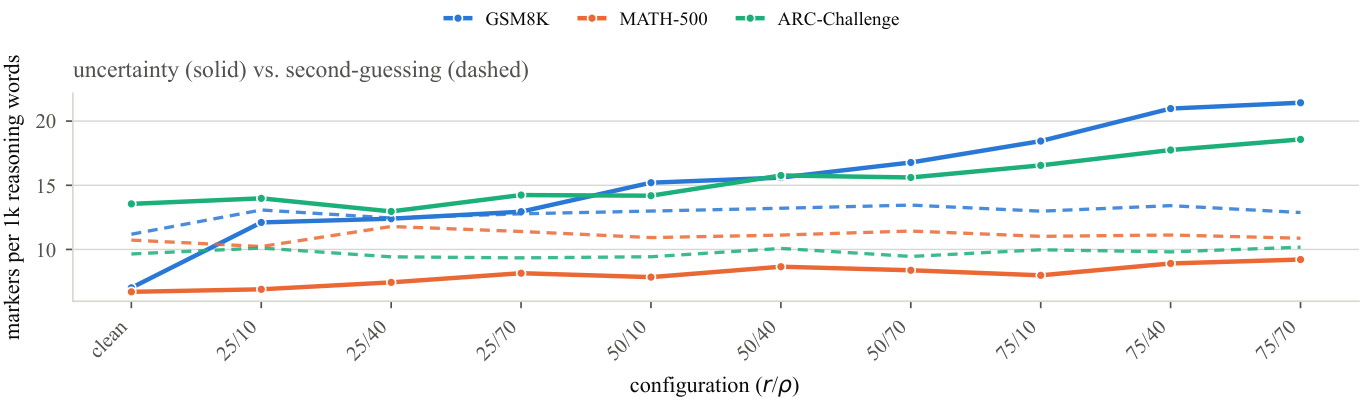
\includegraphics[width=\textwidth]{figures/fig5_doubt.png}
\caption{\textbf{Self-doubt under typos.} Marker density per 1,000 reasoning words across the grid. Uncertainty markers (solid) rise with corruption on all three datasets, most steeply on GSM8K, while second-guessing markers (dashed) stay roughly flat: typos make the model express more doubt without making it verify more. The same densities split by final answer are in Table 7.}
\label{fig:5}
\end{figure*}


\subsection{No lightweight mitigation reliably helps}

We tested the three mitigation strategies from our plan on GSM8K (Table 3).

\paragraph{Warn.} Prefixing the prompt with ``Note: the text may contain typos.'' changed accuracy by only $-$1.0 percentage points on average across the nine typo conditions, with effects ranging from $-$4.3 to +1.2 points. This is consistent with \S5.3, where the model often already showed signs of noticing that the input was corrupted: the limitation does not appear to be awareness of the typo itself.

\paragraph{Rewrite.} Instructing the model to first rewrite the question with the typos corrected and only then solve it performed worse than the original prompt in all nine conditions, reducing accuracy by 5.2 percentage points on average and by up to 7.6 points. Median reasoning length also fell, from about 1,300 to about 740 tokens (median over the nine typo conditions). One possible explanation is that the rewrite step forces the model to commit to a single interpretation of the corrupted question too early; if the reconstruction is wrong, the model reasons about the wrong problem with little opportunity to recover.

\paragraph{Spell check.} We applied an external spell checker (\texttt{pyspellchecker}, edit distance 2, prose words only) to the same questions before sending them to the model. A typo counts as recovered only if it is restored exactly to the original word. Recovery dropped as the share of real-word typos increased: from 55.0\% at $\rho$=10 to 39.9\% at $\rho$=40 and 25.8\% at $\rho$=70 (pooled over all corrupted words). This lexical recovery did not translate into a consistent accuracy gain: the spell checker changed accuracy by $-$0.6 percentage points on average, improving four conditions and hurting five, including the hardest one (62.2\% against 64.5\% without it). Spell checkers detect non-word errors far better than real-word substitutions, and may even replace a non-word typo with a wrong valid word, creating the kind of error that \S5.2 found to be more harmful.

\begin{table}[t]
\centering
\small
\resizebox{\columnwidth}{!}{%
\begin{tabular}{lrrrrrrr}
\toprule
 & \textbf{no fix} & \multicolumn{2}{c}{\textbf{warn}} & \multicolumn{2}{c}{\textbf{rewrite}} & \multicolumn{2}{c}{\textbf{spell check}} \\
\cmidrule(lr){3-4}\cmidrule(lr){5-6}\cmidrule(lr){7-8}
\textbf{r/$\rho$} & acc & acc & $\Delta$ & acc & $\Delta$ & acc & $\Delta$ \\
\midrule
25/10 & 85.5 & 85.7 & +0.2 & 83.8 & -1.7 & 87.0 & +1.5 \\
25/40 & 87.0 & 87.2 & +0.2 & 82.9 & -4.1 & 86.1 & -0.9 \\
25/70 & 86.7 & 85.5 & -1.2 & 80.2 & -6.6 & 85.3 & -1.4 \\
50/10 & 79.6 & 79.4 & -0.2 & 76.4 & -3.2 & 79.0 & -0.6 \\
50/40 & 79.0 & 74.7 & -4.3 & 71.5 & -7.5 & 75.1 & -3.9 \\
50/70 & 72.8 & 74.0 & +1.2 & 67.9 & -4.9 & 73.2 & +0.4 \\
75/10 & 74.2 & 70.6 & -3.7 & 66.9 & -7.4 & 75.3 & +1.0 \\
75/40 & 67.3 & 66.3 & -1.0 & 63.8 & -3.5 & 68.1 & +0.9 \\
75/70 & 64.5 & 63.9 & -0.6 & 56.9 & -7.6 & 62.2 & -2.3 \\
\midrule
\textbf{mean} &  &  & \textbf{-1.0} &  & \textbf{-5.2} &  & \textbf{-0.6} \\
\bottomrule
\end{tabular}}
\caption{GSM8K answered-only accuracy (\%) under each mitigation, per condition, with the change against the unmodified prompt (\emph{no fix}). The mean row is taken over the nine typo conditions. $\Delta$ is computed from unrounded accuracies, so it can differ by 0.1 from the difference of the values shown.}
\label{tab:3}
\end{table}


\section{Discussion}

The most consistent finding across our analyses is that real-word typos are more harmful than non-word typos, in the per-typo regression, the paired comparisons, and the spell-checker results. One might expect the opposite, since non-word typos disrupt tokenization. Our results suggest that a non-word typo is visibly unusual and signals that something is wrong, whereas a real-word typo is fluent, tokenized normally, and may fit the sentence well enough that its wrong meaning is taken at face value. The same property makes it hard for dictionary-based correction, which can only act on forms that are not valid words.

The trace analysis points to a related conclusion. The model often notices that the input is unusual: uncertainty language increases, corrupted words are flagged more often, and traces become longer. This additional effort does not reliably lead to recovery, which also explains why the mitigations had little effect: a warning adds information the model often already has, while a forced rewrite commits it early to a single, possibly wrong, interpretation. The main difficulty is therefore not detecting that a typo exists, but recovering the intended word when the corruption is ambiguous. A more promising direction may be to keep multiple interpretations open during reasoning and resolve them later using the structure of the problem. Finally, longer traces should not be read as evidence of successful self-correction: incorrect answers produce longer traces even on clean input.


\section{Limitations}

\paragraph{One model, one sample.} All headline results come from a single 7B reasoning model at one decoding setting with n=1 sample per question. Our plan called for several samples per question, but the API budget did not permit it, so we cannot separate typo effects from decoding variance at the level of an individual question. The overall effects are much larger than expected sampling noise (McNemar p $<$ 10$^{-6}$ on n=482 paired items), but generalization to larger reasoning models is untested.

\paragraph{Dataset substitution.} We replaced the planned GPQA-Diamond \citep{rein2024} with ARC-Challenge, another multiple-choice science dataset. On clean GPQA-Diamond the model reached only about 52\% accuracy against a 25\% chance level, which leaves little room to measure further drops before changes reflect guessing rather than reasoning. ARC-Challenge is easier and its answer options may help the model recover information, so our multiple-choice results may underestimate the effect of typos on harder science questions.

\paragraph{Scope of the mitigation study.} We tested the mitigations only on GSM8K, because each required additional paid API calls; we chose GSM8K because it showed the clearest drop under typos, making it the most informative dataset for testing whether a mitigation recovers performance.


\section{AI Disclosure and Reflection}

\paragraph{What we used AI for.} We used GitHub Copilot with Claude primarily to support coding tasks during the project. It helped us build the typo-generation and inference pipelines, write analysis scripts, generate matplotlib code for figures, and improve the wording of some parts of the paper. All methodological and experimental decisions, including the two-axis corruption grid, typo-type weights, answer-extraction rules, and judge rubric, were made by us. The analysis scripts were written with Claude's assistance based on these decisions, and all reported results were generated from the raw generation logs using those scripts.

\paragraph{Reflection.} AI tools were especially useful for speeding up repetitive coding and analysis tasks and for keeping the implementation consistent across experiments. However, generated code and outputs still required careful checking, particularly for numerical results. We therefore verified reported results against the raw data and used a consistent scoring procedure throughout the analysis. Overall, the project highlighted the importance of reproducibility and independent verification when AI tools are used in research.


\section{Conclusion}

Typos have a clear and consistent effect on reasoning performance. On GSM8K, accuracy dropped by as much as 28.1 percentage points, with larger declines as the corruption rate increased, and the strongest effect came from typos that turned one valid English word into another. The main problem is not that the model fails to notice corrupted input: it often recognizes that something is wrong, but cannot reliably recover the intended meaning. Its traces show more uncertainty rather than more verification, and neither prompting strategies nor dictionary-based correction consistently improved performance. Robustness to everyday typing errors should therefore be treated as a capability to be developed explicitly, rather than assumed from strong benchmark performance.

All code is available in the project repository, and the raw generation logs are hosted on the Hugging Face Hub (\texttt{ronshtricker/typo-reasoning-results}). All reported results can be reproduced by running \texttt{download\_data.py} followed by \texttt{run\_all.py}.


\bibliography{custom}

\clearpage
\onecolumn
\appendix


\section{Full accuracy grid}

\begin{table}[H]
\centering
\scriptsize
\resizebox{\textwidth}{!}{%
\begin{tabular}{lrrrrrrrrrrrrrrrrrr}
\toprule
 & \multicolumn{6}{c}{\textbf{GSM8K}} & \multicolumn{6}{c}{\textbf{MATH-500}} & \multicolumn{6}{c}{\textbf{ARC-Challenge}} \\
\cmidrule(lr){2-7}\cmidrule(lr){8-13}\cmidrule(lr){14-19}
\textbf{condition} & acc & n\_a & tok & r$\rightarrow$w & w$\rightarrow$r & p & acc & n\_a & tok & r$\rightarrow$w & w$\rightarrow$r & p & acc & n\_a & tok & r$\rightarrow$w & w$\rightarrow$r & p \\
\midrule
clean & 92.6 & 500 & 1535 & -- & -- & -- & 95.2 & 496 & 2927 & -- & -- & -- & 85.2 & 494 & 1167 & -- & -- & -- \\
typo25\_real10 & 85.5 & 497 & 1913 & 48 & 13 & 1.3e-05 & 93.9 & 495 & 2945 & 12 & 7 & 0.359 & 86.2 & 492 & 1218 & 26 & 30 & 0.688 \\
typo25\_real40 & 87.0 & 500 & 1814 & 42 & 14 & 3.1e-04 & 93.4 & 498 & 3111 & 15 & 9 & 0.307 & 86.2 & 493 & 1243 & 27 & 32 & 0.603 \\
typo25\_real70 & 86.7 & 497 & 1843 & 43 & 13 & 1.1e-04 & 93.9 & 494 & 2992 & 15 & 9 & 0.307 & 82.4 & 495 & 1239 & 41 & 26 & 0.087 \\
typo50\_real10 & 79.6 & 500 & 2024 & 80 & 15 & $<$1e-6 & 92.8 & 498 & 2939 & 18 & 9 & 0.124 & 82.2 & 490 & 1296 & 42 & 28 & 0.120 \\
typo50\_real40 & 79.0 & 500 & 2084 & 84 & 16 & $<$1e-6 & 91.4 & 498 & 3085 & 22 & 6 & 0.005 & 82.4 & 493 & 1359 & 42 & 25 & 0.051 \\
typo50\_real70 & 72.8 & 500 & 2094 & 110 & 11 & $<$1e-6 & 91.5 & 496 & 3087 & 25 & 9 & 0.010 & 82.7 & 490 & 1325 & 44 & 30 & 0.131 \\
typo75\_real10 & 74.2 & 489 & 2104 & 101 & 9 & $<$1e-6 & 89.1 & 494 & 2945 & 34 & 5 & 7.3e-06 & 81.0 & 490 & 1383 & 56 & 35 & 0.036 \\
typo75\_real40 & 67.3 & 495 & 2593 & 138 & 13 & $<$1e-6 & 88.1 & 496 & 3125 & 39 & 7 & 4.9e-06 & 77.5 & 489 & 1408 & 65 & 28 & 1.9e-04 \\
typo75\_real70 & 64.5 & 482 & 2330 & 148 & 11 & $<$1e-6 & 86.9 & 497 & 3137 & 46 & 7 & $<$1e-6 & 74.5 & 490 & 1447 & 77 & 25 & $<$1e-6 \\
\bottomrule
\end{tabular}}
\caption{Every condition on every dataset. \emph{acc} is answered-only accuracy (\%), n\_a the number of questions that produced a final answer, \emph{tok} the mean generated tokens. r$\rightarrow$w and w$\rightarrow$r are paired right-to-wrong and wrong-to-right flips against the clean condition over jointly answered questions, with the continuity-corrected McNemar p-value (uncorrected for multiple comparisons).}
\label{tab:4}
\end{table}


\section{Per-typo logistic fit}

\begin{table}[H]
\centering
\small
\begin{tabular}{lrrr}
\toprule
 & \textbf{GSM8K} & \textbf{MATH-500} & \textbf{ARC-C} \\
\midrule
traces in the fit, n & 4460 & 4466 & 4422 \\
intercept & +2.091 & +3.019 & +1.686 \\
coefficient, real-word & -0.0705 & -0.0761 & -0.0428 \\
coefficient, non-word & -0.0402 & -0.0588 & -0.0081 \\
odds multiplier, real-word & 0.932 & 0.927 & 0.958 \\
odds multiplier, non-word & 0.961 & 0.943 & 0.992 \\
odds lost per real-word typo & 6.8\% & 7.3\% & 4.2\% \\
odds lost per non-word typo & 3.9\% & 5.7\% & 0.8\% \\
\textbf{relative loss, real / non-word} & \textbf{1.7$\times$} & \textbf{1.3$\times$} & \textbf{5.2$\times$} \\
95\% CI of the relative loss (bootstrap over questions) & [1.4, 2.3] & [1.0, 1.7] & n/a$^\dagger$ \\
non-word coefficient, 95\% CI & [-0.0528, -0.0284] & [-0.0792, -0.0398] & [-0.0272, +0.0118] \\
\bottomrule
\end{tabular}
\caption{Per-typo logistic fit behind \S5.2. One regression per dataset, correct $\sim$ num\_real + num\_nonword, fitted over all answered typo traces pooled across the nine conditions. The predictors are the counts of each kind of typo actually applied to that question. An odds multiplier is exp(coefficient): the factor by which one additional typo of that kind multiplies the odds of a correct answer. $^\dagger$ On ARC the non-word coefficient's CI includes 0, so the ratio has no finite interval; the difference of the two coefficients is $-$0.035 (95\% CI $-$0.057 to $-$0.012, p=0.003).}
\label{tab:5}
\end{table}


\section{Paired real-word contrasts}

\begin{table}[H]
\centering
\scriptsize
\resizebox{\textwidth}{!}{%
\begin{tabular}{llrrrrrrrrr}
\toprule
 &  & \multicolumn{3}{c}{\textbf{GSM8K}} & \multicolumn{3}{c}{\textbf{MATH-500}} & \multicolumn{3}{c}{\textbf{ARC-Challenge}} \\
\cmidrule(lr){3-5}\cmidrule(lr){6-8}\cmidrule(lr){9-11}
\textbf{r} & \textbf{$\rho$} & $\Delta$acc & r/w & p & $\Delta$acc & r/w & p & $\Delta$acc & r/w & p \\
\midrule
25 & 10$\rightarrow$70 & +1.0 & 31/36 & 0.625 & +0.0 & 10/10 & 1.000 & -3.1 & 45/30 & 0.106 \\
25 & 10$\rightarrow$40 & +1.4 & 28/35 & 0.450 & +0.0 & 10/10 & 1.000 & +0.2 & 32/33 & 1.000 \\
25 & 40$\rightarrow$70 & -0.4 & 30/28 & 0.896 & -0.2 & 13/12 & 1.000 & -4.1* & 41/21 & 0.016 \\
50 & 10$\rightarrow$70 & -6.8* & 76/42 & 0.002 & -1.4 & 19/12 & 0.281 & +0.4 & 41/43 & 0.913 \\
50 & 10$\rightarrow$40 & -0.6 & 45/42 & 0.830 & -1.4 & 17/10 & 0.248 & +0.2 & 36/37 & 1.000 \\
50 & 40$\rightarrow$70 & -6.2* & 70/39 & 0.004 & -0.2 & 13/12 & 1.000 & +0.2 & 37/38 & 1.000 \\
75 & 10$\rightarrow$70 & -11.0* & 94/42 & 1.2e-05 & -1.8 & 28/19 & 0.243 & -6.9* & 61/28 & 6.9e-04 \\
75 & 10$\rightarrow$40 & -6.2* & 87/57 & 0.016 & -0.2 & 20/19 & 1.000 & -4.0 & 52/33 & 0.051 \\
75 & 40$\rightarrow$70 & -3.6 & 74/57 & 0.162 & -1.6 & 25/17 & 0.280 & -3.1 & 60/45 & 0.172 \\
\bottomrule
\end{tabular}}
\caption{Controlled paired contrast behind \S5.2, at every typo rate and every pair of real-word ratios. Within a fixed r the same words of the same questions are corrupted in the same positions, so only the \emph{kind} of corruption changes. $\Delta$acc is the accuracy of the higher-$\rho$ variant minus the lower, over questions answered in both; \emph{r/w} is right-to-wrong against wrong-to-right flips; p is a continuity-corrected McNemar test and * marks p$<$0.05 before multiple-comparison correction.}
\label{tab:6}
\end{table}


\section{Reasoning length and self-doubt markers}

\begin{table}[H]
\centering
\scriptsize
\resizebox{\textwidth}{!}{%
\begin{tabular}{lrrrrrrrrrrrrrrrrrr}
\toprule
 & \multicolumn{6}{c}{\textbf{GSM8K}} & \multicolumn{6}{c}{\textbf{MATH-500}} & \multicolumn{6}{c}{\textbf{ARC-Challenge}} \\
\cmidrule(lr){2-7}\cmidrule(lr){8-13}\cmidrule(lr){14-19}
\textbf{condition} & tok & tok\_c & tok\_w & uncert. & 2nd-g. & u.w/c & tok & tok\_c & tok\_w & uncert. & 2nd-g. & u.w/c & tok & tok\_c & tok\_w & uncert. & 2nd-g. & u.w/c \\
\midrule
clean & 1535 & 1412 & 3082 & 7.0 & 11.2 & 1.59 & 2927 & 2803 & 5352 & 6.7 & 10.7 & 1.70 & 1167 & 1018 & 2026 & 13.6 & 9.7 & 1.71 \\
typo25\_real10 & 1913 & 1511 & 4281 & 12.1 & 13.1 & 1.83 & 2945 & 2826 & 4783 & 6.9 & 10.2 & 1.61 & 1218 & 1118 & 1837 & 14.0 & 10.1 & 1.57 \\
typo25\_real40 & 1814 & 1567 & 3471 & 12.4 & 12.5 & 1.90 & 3111 & 2900 & 6075 & 7.4 & 11.8 & 1.52 & 1243 & 1111 & 2069 & 13.0 & 9.4 & 1.72 \\
typo25\_real70 & 1843 & 1537 & 3843 & 12.9 & 12.8 & 2.12 & 2992 & 2859 & 5047 & 8.2 & 11.4 & 1.66 & 1239 & 1073 & 2015 & 14.2 & 9.3 & 1.91 \\
typo50\_real10 & 2024 & 1554 & 3856 & 15.2 & 13.0 & 1.87 & 2939 & 2763 & 5191 & 7.8 & 10.9 & 1.97 & 1296 & 1182 & 1828 & 14.2 & 9.4 & 1.51 \\
typo50\_real40 & 2084 & 1631 & 3787 & 15.6 & 13.2 & 1.64 & 3085 & 2839 & 5694 & 8.7 & 11.1 & 1.96 & 1359 & 1214 & 2037 & 15.8 & 10.1 & 1.91 \\
typo50\_real70 & 2094 & 1501 & 3682 & 16.8 & 13.5 & 1.66 & 3087 & 2854 & 5600 & 8.4 & 11.4 & 1.90 & 1325 & 1176 & 2033 & 15.6 & 9.5 & 1.66 \\
typo75\_real10 & 2104 & 1598 & 3559 & 18.4 & 13.0 & 1.60 & 2945 & 2787 & 4236 & 8.0 & 11.0 & 2.05 & 1383 & 1236 & 2012 & 16.6 & 10.0 & 1.48 \\
typo75\_real40 & 2593 & 1786 & 4253 & 21.0 & 13.4 & 1.60 & 3125 & 2881 & 4932 & 8.9 & 11.1 & 2.06 & 1408 & 1260 & 1919 & 17.8 & 9.8 & 1.40 \\
typo75\_real70 & 2330 & 1638 & 3588 & 21.4 & 12.9 & 1.63 & 3137 & 2911 & 4640 & 9.2 & 10.9 & 1.75 & 1447 & 1260 & 1995 & 18.6 & 10.2 & 1.47 \\
\bottomrule
\end{tabular}}
\caption{Supporting numbers for \S5.1 and \S5.4. \emph{tok} is mean generated tokens over all answered traces; \emph{tok}\_c and \emph{tok}\_w are the same mean over traces that ended in a correct and in a wrong answer. \emph{uncert.} and \emph{2nd-g.} are uncertainty and second-guessing markers per 1,000 reasoning words, and \emph{u.w/c} is uncertainty density in wrong-answer traces divided by correct-answer traces. Traces generally lengthen with the typo rate (MATH-500 at $\rho$=10 and $\rho$=40 is flat), a wrong answer is preceded by a longer trace than a correct one in every condition, and uncertainty climbs while second-guessing stays roughly flat.}
\label{tab:7}
\end{table}


\section{Word-level repair behaviour}

\begin{table}[H]
\centering
\scriptsize
\resizebox{\textwidth}{!}{%
\begin{tabular}{llrrrrrrrrrrrrrrrrrr}
\toprule
 &  & \multicolumn{6}{c}{\textbf{GSM8K}} & \multicolumn{6}{c}{\textbf{MATH-500}} & \multicolumn{6}{c}{\textbf{ARC-Challenge}} \\
\cmidrule(lr){3-8}\cmidrule(lr){9-14}\cmidrule(lr){15-20}
\textbf{r} & \textbf{$\rho$} & silent & flag & mis. & unused & mis\_c & mis\_w & silent & flag & mis. & unused & mis\_c & mis\_w & silent & flag & mis. & unused & mis\_c & mis\_w \\
\midrule
25 & 10 & 74.0 & 11.3 & 2.9 & 11.9 & 2.5 & 5.0 & 77.7 & 1.7 & 1.2 & 19.3 & 1.3 & 0.4 & 80.8 & 5.2 & 1.9 & 12.0 & 1.6 & 3.8 \\
25 & 40 & 72.4 & 12.9 & 4.1 & 10.5 & 3.8 & 6.3 & 74.5 & 3.3 & 1.5 & 20.7 & 1.2 & 3.4 & 76.9 & 7.0 & 2.6 & 13.5 & 2.1 & 5.1 \\
25 & 70 & 68.1 & 15.4 & 4.7 & 11.8 & 4.2 & 7.8 & 75.0 & 5.6 & 1.5 & 17.9 & 1.3 & 3.4 & 73.3 & 9.1 & 4.1 & 13.4 & 3.7 & 5.7 \\
50 & 10 & 66.3 & 18.4 & 4.6 & 10.7 & 3.7 & 7.5 & 75.1 & 3.6 & 1.4 & 19.9 & 1.2 & 2.5 & 77.5 & 7.6 & 2.4 & 12.5 & 1.8 & 4.9 \\
50 & 40 & 62.6 & 21.4 & 5.0 & 11.0 & 4.8 & 5.7 & 71.2 & 6.0 & 2.1 & 20.7 & 2.0 & 2.7 & 74.0 & 9.6 & 3.4 & 13.1 & 3.0 & 4.7 \\
50 & 70 & 59.0 & 22.0 & 6.3 & 12.7 & 5.9 & 7.3 & 70.5 & 6.9 & 2.6 & 20.0 & 2.1 & 5.3 & 70.3 & 10.9 & 4.7 & 14.1 & 4.5 & 5.6 \\
75 & 10 & 55.8 & 26.9 & 6.5 & 10.8 & 5.8 & 8.2 & 70.6 & 7.6 & 2.0 & 19.8 & 1.6 & 3.4 & 71.9 & 12.7 & 3.2 & 12.1 & 2.8 & 5.0 \\
75 & 40 & 48.8 & 32.3 & 7.8 & 11.2 & 6.1 & 10.7 & 69.9 & 7.3 & 2.3 & 20.5 & 1.6 & 4.8 & 67.9 & 14.5 & 4.5 & 13.1 & 4.1 & 5.8 \\
75 & 70 & 48.3 & 29.4 & 9.2 & 13.0 & 7.8 & 11.5 & 65.1 & 11.0 & 3.7 & 20.2 & 3.1 & 5.7 & 62.5 & 17.2 & 6.2 & 14.0 & 5.3 & 8.9 \\
\bottomrule
\end{tabular}}
\caption{Every corrupted word in every condition, classified by how the reasoning trace handles it, as a percentage of the corrupted words in that condition. \emph{silent} / \emph{flag} / \emph{mis.} / \emph{unused} are the four categories of \S5.3. \emph{mis}\_c and \emph{mis}\_w are the misread rate among questions the model answered correctly and among those it answered wrongly, which is the comparison behind the claim that misreading is associated with failure. Figure 4 shows the same data pooled along each axis. Words whose corrupted form also appears in the model's trace on the clean question (about 3\% overall) are left out.}
\label{tab:8}
\end{table}


\section{Responses that reach the token limit}

\begin{table}[H]
\centering
\small
\begin{tabular}{lrrr}
\toprule
\textbf{condition} & \textbf{GSM8K} & \textbf{MATH-500} & \textbf{ARC-Challenge} \\
\midrule
clean & 0 & 4 & 6 \\
typo25\_real10 & 3 & 5 & 8 \\
typo25\_real40 & 0 & 2 & 7 \\
typo25\_real70 & 3 & 6 & 5 \\
typo50\_real10 & 0 & 2 & 10 \\
typo50\_real40 & 0 & 2 & 7 \\
typo50\_real70 & 0 & 4 & 10 \\
typo75\_real10 & 11 & 6 & 10 \\
typo75\_real40 & 5 & 4 & 10 \\
typo75\_real70 & 17 & 3 & 10 \\
\midrule
\textbf{all ten} & 39 \textbf{(0.8\%)} & \textbf{38 (0.8\%)} & \textbf{83 (1.7\%)} \\
\bottomrule
\end{tabular}
\caption{Responses that reach the generation cap (20,000 tokens for GSM8K, 17,000 for MATH-500 and ARC-Challenge), out of 500 questions per condition; the last row is out of 5,000. None of them contains a final answer, so all are counted as unanswered. At most 17 of 500 (3.4\%) reach the cap in any condition. The remaining unanswered responses in Table 4 stopped before the cap without an extractable answer.}
\label{tab:9}
\end{table}

\end{document}
